\begin{figure}[h]
    \centering
    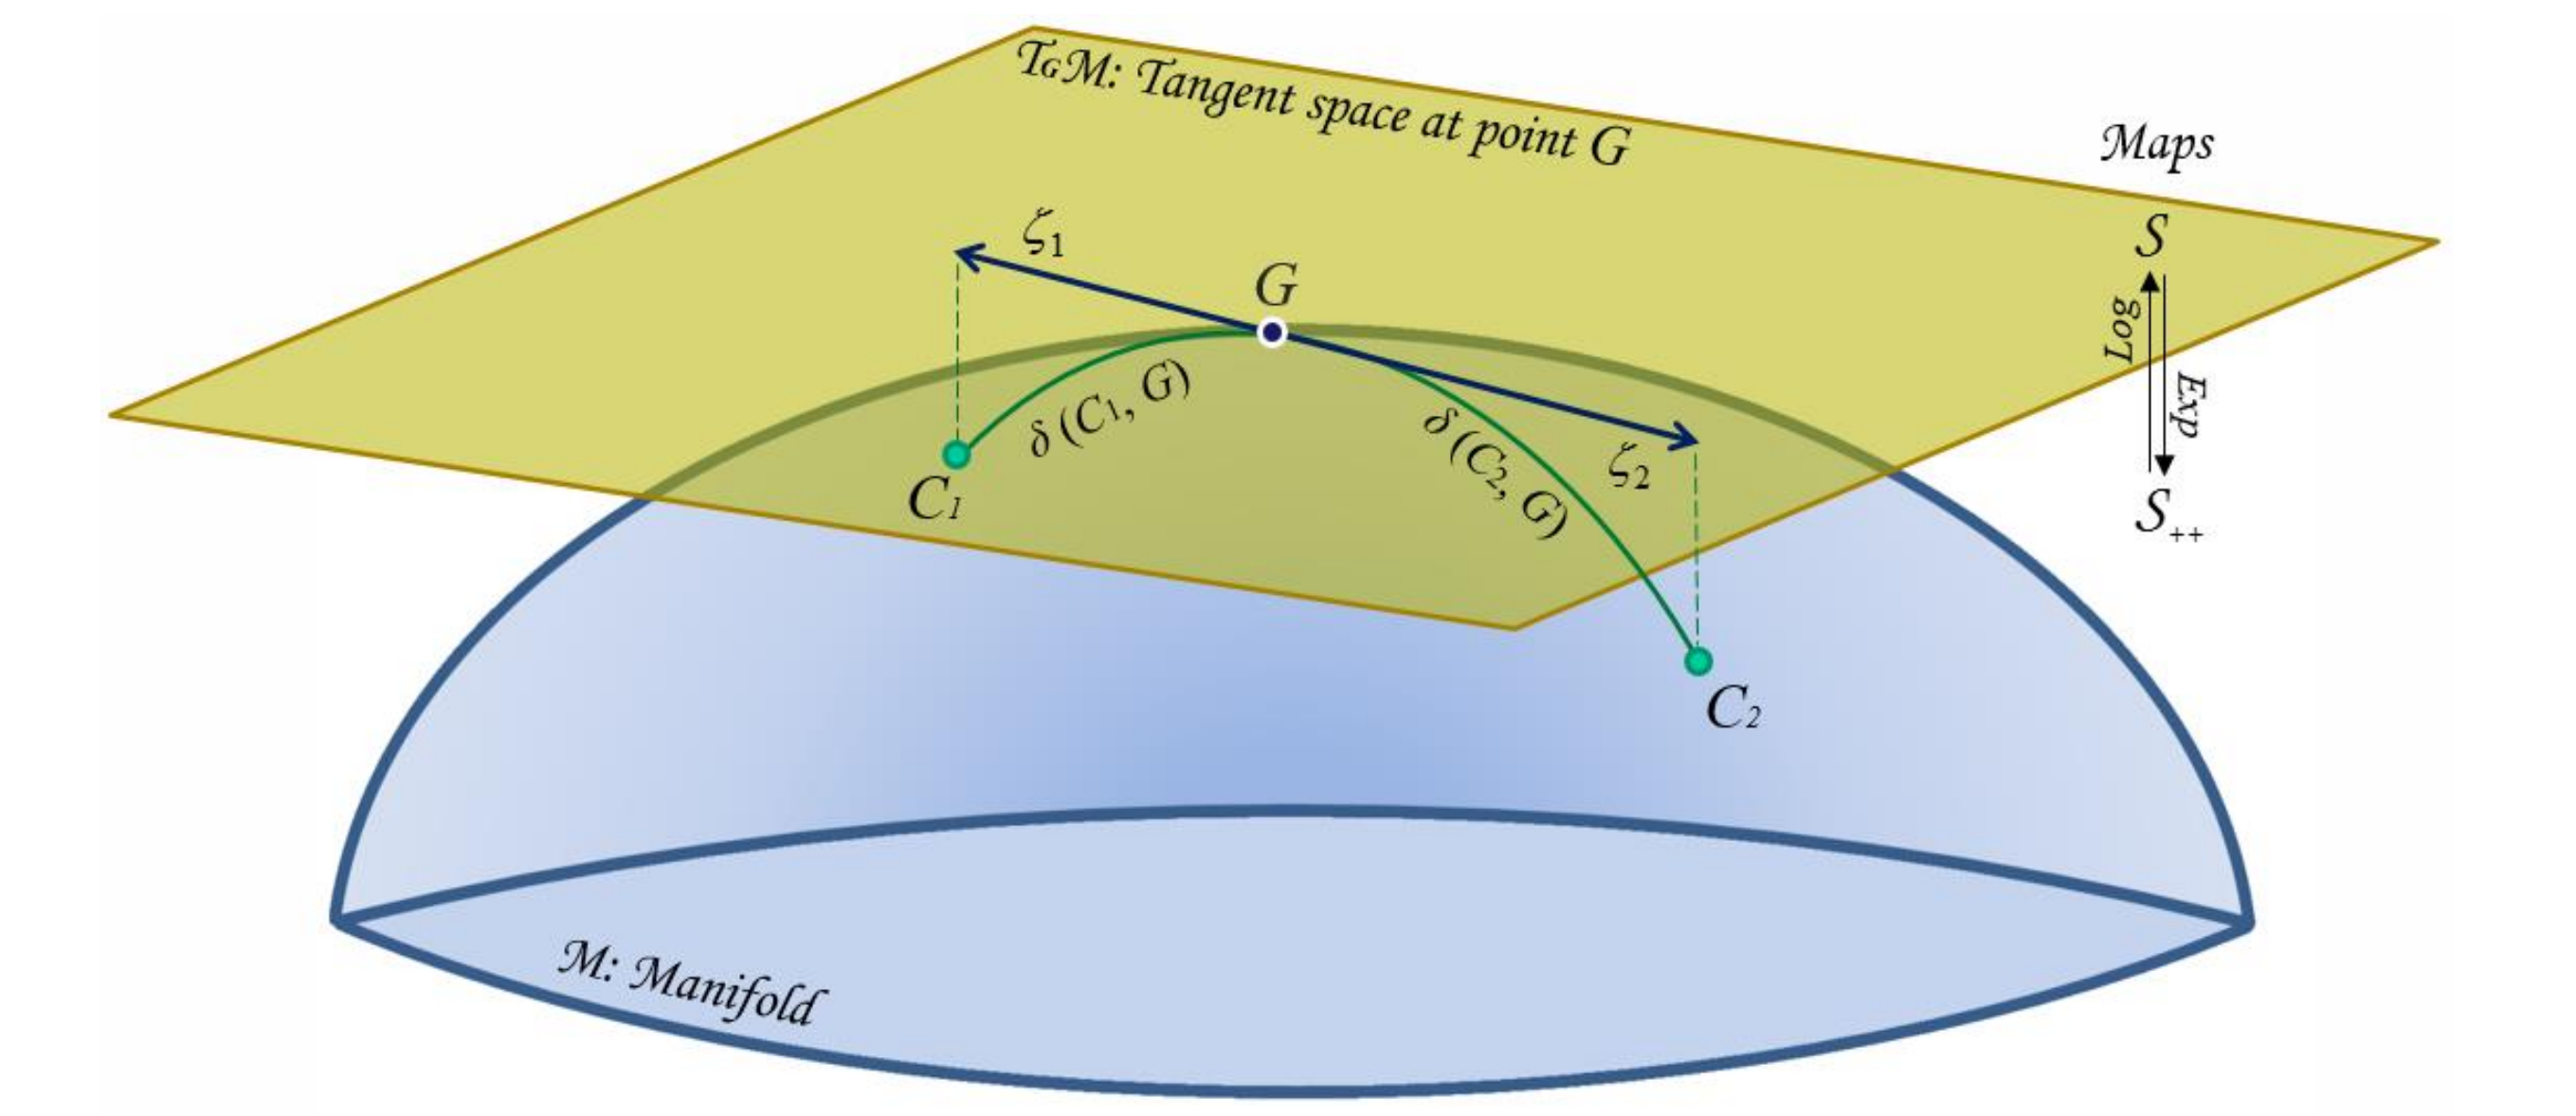
\includegraphics[width=0.6\textwidth]{img/riemannian-tangent-space.png}
    \caption{Schematic representation of the symmetric positive definite matrix manifold, the geometric mean $G$ of two points and the tangent space at $G$. The geometric mean of these points is the midpoint on the geodesic connecting $C_1$ and $C_2$, i.e.\ it minimizes the sum of the two squared distances. The map from the tangent space to the manifold is an exponential map. The inverse map is a logarithmic map.}\label{figure:tangent-space}
    \source{Congedo et al.~\cite{congedo_riemannian_2017}}
\end{figure}
